
\newrefcontext[sorting=ynt]

    \lettrine{A}{nimal} movement is understood to be an individual response that integrates multiple internal and external stimuli, including environmental conditions and the presence of other animals \citep{nathan2008a}.
    Various aspects of animal movement, such as the distance moved over time (speed), or the tortuosity of an animal's path, are now readily measured and quantified in free-living individuals, given significant advances in animal tracking technology \citep[][see Nathan et al. \textit{in prep.}]{cagnacci2010}.
    This makes movement a sort of `model behaviour' that allows investigation of the underlying mechanisms --- the `how' and `why' of animal decision-making --- under natural conditions that cannot be replicated in experimental settings.
    For example, tracking individual greenbuls \textit{Phyllastrephus sp.} in forested landscapes revealed that greenbuls moved more frequently to trees that were actually visible from their position, rather than trees that were obscured from view, indicating that visual cues are important in the movement decisions of forest birds \citep[][see also \citep{aben2018}]{aben2021}.
    This illustrates a general tactic in animal movement studies, which is to treat an animal's use of a resource disproportionate to its availability \citep{manly2007,fortin2005,signer2019}, or prolonged residence in an area \citep{bracis2018} as indicators of adaptive movement decision-making mechanisms.
    Simple simulation models show that differences in movement patterns --- such as path metrics, or emergent social interactions --- may reflect underlying differences in movement strategies \citep{spiegel2017}.
    
    Both differences in movement strategies, or the mechanisms controlling movement \citep{spiegel2017}, and differences in movement paths, which are the outcomes of movement mechansims \citep{abrahms2017,hertel2021}, are interpreted as facets of animal personality \citep{sih2004,sih2004a}.
    Increasingly however, animal personality, or consistent individual differences in behaviour, are studied in empirical terms, and considered to be detected in a population when its behavioural responses possess certain statistical properties \citep{sanchez-tojar2021}.
    In the context of animal movement, researchers apply sophisticated variance-partitioning approaches to common movement metrics --- such as daily distance moved --- and aim to determine how much behavioural variation in a population is explained by individual identity, rather than conditions that directly influence behaviour (e.g. diel cycle, temperature), or variation due to other, un-examined factors (e.g. weather differences between intervals) \citep{hertel2020, hertel2019, hertel2021}.
    Another approach to investigate individual animals' decision-making mechanisms is to estimate their relative preferences for environmental conditions using step-selection analysis \citep[][see also resource selection analysis: \citealt{manly2007}]{fortin2005,thurfjell2014,avgar2016,signer2019,fieberg2021}.
    Step-selection analysis compares environmental cues between animals' real steps --- the movements actually made, and their alternatives --- the movements that \textit{could have been made}, from the same starting location \citep{thurfjell2014,fieberg2021}.
    The relative selection strengths, which are the coefficients of a step-selection function, can be compared between individuals \citep{thurfjell2014}, and should be expected to be different for individuals with different movement decision-making mechanisms.
    
    However, it is unclear whether individual consistency in the mechanisms underlying movement strategies can really be identified using current statistical tools.
    Most researchers realise that there is a substantial gap between the environment animals perceive and to which they respond, and the often static representation of that environment that is measured in tracking studies.
    For example, resources that are critical to animals are often ephemeral, and difficult to measure with both a high spatio-temporal extent and resolution using existing technologies such as remote sensing, leading researchers to fall back on more long-term resource proxies such as vegetation indices \citep{pettorelli2011}.
    This issue is likely even more acute in the case of movements that have a social context, such as competition, as the social environment is expected to change even more rapidly than resource distributions, and to be even more sensitive to local consumer densities.
    Consequently, it may be difficult to determine whether differences in movement reflect underlying differences in decision-making mechanisms, or whether they better represent stochastic differences in environmental conditions encountered by animals.
    Applying current methods in animal movement ecology to individual-based simulation models of animal movement strategies \citep[see e.g.][]{getz2015,getz2016,netz2020,gupte2021a}can help explore whether these methods can reliably detect individual differences in movement decision-making mechanisms.
    
    Mechanistic models of intermediate complexity can simulate the main features of many spatial systems, such as heterogeneity in landscape productivity, and resource depletion due to mobile consumers \citep{getz2015,white2018,deangelis2019,netz2020,gupte2021a,diaz2021}.
    Here, we work with an evolutionary, individual-based model of agent movement in the context of intraspecific competition \citep[both exploitation and interference]{gupte2021a}.
    In our model, agent movement is the outcome of the interplay of simple movement decision-making mechanisms, a fluctuating resource landscape, and due to agent movement, a variable social landscape.
    % Agents can be programmed to move according to specific movement rules, which are controlled by 
    Agent movement strategies are controlled by their preferences for environmental cues, such as resource and competitor densities \citep[see e.g.][]{getz2015,white2018,netz2020, gupte2021a}.
    % The movement weights are used to assess the fluctuating resource landscape, as well as changing local densities of competitors.
    These preferences may be thought of as the coefficients of resource- or step-selection functions \citep[][]{white2018,gupte2021a}.
    Importantly, in contrast with purely ecological models \citep[e.g.][]{white2018}, agents' preferences are outcomes of many generations of natural selection \citep[see also][]{getz2015,netz2020}.
    We previously showed that in two scenarios of exploitation and interference competition, differences among individuals in how they assess local environmental cues evolve \citep[][]{gupte2021a}.
    % Consequently, we would expect to see these differences in mechanisms reflected in the structure of emergent movement paths.
    
    We tackle three specific aspects of a general question in animal movement: what can applying statistical tools to animal tracking data tell us about individual differences in the movement decision-making mechanisms?
    \textit{(1)} We first examine whether different movement types are indicated by simple exploratory data analysis.
    \textit{(2)} We then investigate the results of a variance-partitioning approach (repeatability analysis; \citealt{nakagawa2010,hertel2019}) to detecting individual differences in populations with different movement types \textit{and} competition strategies.
    % \textit{(2)} Are decision-making mechanisms good predictors of the structure of the paths they generate? Can environmental predictors better explain movement path structure?
    \textit{(3)} Finally, we attempt a novel application of step-selection analysis to the study of consistent individual differences in movement strategies.
    Overall, by treating a simulation model with simple movement rules as we would empirical animal-tracking data, we aim to explore whether individual differences in movement decision-making mechanisms can be reliably inferred from the emergent structure of animal movement paths.
    
    \section{Methods}
    
    \subsection*{The Model}
    
    We worked with an individual-based evolutionary simulation model of animal movement in a foraging context (\textit{Charadrii}; \citealt{gupte2021a}; model code: \citealt{netz2022a}).
    We describe the model's ecological dynamics in brief here, and refer readers to \cite{gupte2021a} for a more detailed exploration of the evolutionary outcomes.
    
    \paragraph*{Model Setup and Landscape}
    
    Our model simulates a population with a fixed size (10,000 individuals), moving on a finely gridded landscape of 512\textsuperscript{2} cells; this is a population density of 1 individual for every 26 cells.
    The landscape is wrapped at the boundaries so that individuals passing beyond the bounds at one end re-appear on the diametrically opposite side.
    The model consists of $G$ generations (default = 250) of $T$ timesteps (default = 400); in each generation, individuals move and make foraging decisions to gain intake.
    % , and is also an important mechanism influencing the structure of individual movement paths.
    At the end of each generation, individuals reproduce and pass on their movement and foraging strategies to their offspring, the number of which is proportional to their intake in the 400 timesteps of their `lifetime'.
    
    The cells of the gridded landscape each have a cell-specific probability $r$ of generating a discrete resource, which we refer to as `prey items' (e.g. a mussel).
    The cells are arranged into 1,024 regularly spaced clusters, or `resource peaks', in which the productivity of cells at the centre of the peak (called $r_{max}$) is five times greater than the cells at the periphery of the peak; resource peaks are approximately 16 cells away from each other (see {\color{red}Supplementary Material Fig. S1}).
    We ran the model with a default $r_{max}$ of 0.01, and also at $r_{max}$ values between 0.001 and 0.03, to examine the effect of landscape.
    For an $r_{max}$ = 0.01, the most productive cells (at the centres of a cluster) are likely to generate one item per 100 timesteps (or four items per generation, for $T$ = 400), while the least productive cells (at cluster peripheries) are likely to generate one item every 500 timesteps ($<$ than one item per generation, for $T$ = 400).
    Cells in our landscape were modelled as having a uniform carrying capacity $K$ of 5 prey items, and while a cell is at carrying capacity its $r$ is 0.
    
    \paragraph*{Individual Foraging and Movement}
    
    Agents can perceive a cue indicating the number of all prey items $P$ in a cell, but have a probability $q$ of failing to detect a prey item, and a probability $q^P$ of not detecting any of $P$ prey items; foragers are thus successful in finding a prey item with a probability $1 - q^P$.
    Individuals on a cell forage in a randomised sequence, and the probability of finding a prey item ($1 - q^P$) is updated as individuals find prey, reducing $P$.
    Foragers that are assigned a prey item in timestep $t$ begin handling it, and are considered to be handlers for the next $T_H$ timesteps, during which they are immobile: this creates opportunities for kleptoparasitism \citep{holmgren1995}.
    Foragers that are not assigned a prey item are considered idle, and are counted as non-handlers.
    
    Agent movement is a fine-scale process comprised of small, discrete steps of fixed size.
    These steps are the outcome of short-term individual movement decisions, in which the agent selects a destination cell, after assessing potential destinations based on available cues \citep[similar to step selection or resource selection][]{fortin2005,manly2007}, an approach used previously by \cite{getz2015} and \cite{white2018}.
    In brief, individuals scan the nine cells of their Moore neighbourhood for three environmental cues, \textit{(1)} an indication of the number of discrete prey items $P$, \textit{(2)} the number of individuals handling prey $H$ (called `handlers'), and \textit{(3)} the number of individuals not handling prey $N$ (called `non-handlers').
    Based on these cues, agents rank their neighbouring cells by their `suitability score' $S$, where $S = s_PP + s_HH + s_NN$, and move to the cell to which they have individually assigned the highest suitability.
    The weighing factors for each cue, $s_P$, $s_H$, and $s_N$, are genetically encoded and and transmitted from parents to their offspring.
    All individuals move simultaneously, and then implement their foraging strategy to acquire prey.
    
    \paragraph*{Scenarios of Intraspecific Competition}
    
    We considered two scenarios of intraspecific foraging competition, a process that can strongly shape animal movement and population distributions \citep{fretwell1970,parker1978}.
    %%
    In the exploitation competition \textbf{scenario 1}, agents move about on the landscape according to their movement rules, and find, handle, and consume prey.
    Agents must handle each prey item for a fixed handling time $T_H$ (default = 5) before they gain its energetic value.
    Agents can be either in the handling or searching state \citep{holmgren1995}.
    While handling, agents are immobile and do not make any movements.
    Since there are no direct interactions among agents, the only way in which agents can affect each others' intake is by acquiring prey items before their competitors.
    In this scenario, the only evolvable properties are the environmental cue weighing factors which determine the suitability scores and hence agent movement ($s_P$, $s_H$ and $s_N$).
    
    In \textbf{scenario 2}, agents can either search for prey items (foraging), or steal a prey item from a handler (kleptoparasitism).
    Agents make movement decisions as in the exploitation competition scenario, but their competition strategy (foraging or kleptoparasitism) is fixed through life, genetically encoded, and heritable between generations.
    For simplicity, agents are always successful in stealing from a handler; however, if multiple agents target the same handler, only one of them, randomly selected, is considered successful --- thus kleptoparasitic agents also compete exploitatively among themselves.
    %%
    Handlers that have been stolen from subsequently `flee' and are moved to a random cell within a Chebyshev distance of 5.
    Having acquired prey, a kleptoparasite converts into a handler, but need only handle prey for $T_H - t_h$ timesteps, where $t_h$ is the time that the prey has already been handled by the previous handler; thus kleptoparasites save time on handling compared to a forager.
    Unsuccessful kleptoparasites are considered idle, and are also counted as non-handlers.
    Handlers that finish processing their prey in timestep $t$ return to the non-handler state and are assessed as such by other individuals when determining their movements.
    
    \paragraph*{Inheritance of Movement and Competition Rules}
    
    For simplicity, we modelled discrete, non-overlapping generations, with haploid, asexually reproducing individuals.
    In the exploitation competition scenario, individuals have three active gene loci that encode the decision-making weights which control individual movement ($s_P$, $s_H$, $s_N$). 
    In scenario 2, individuals additionally inherit their competition strategy from their parent.
    % four further weights for foraging decisions ($w_P$, $w_H$, $w_N$, $w_0$) are also active.
    We assume that the expected number of offspring per individual is proportional to the individual's total lifetime intake of resources (hence resource intake is used as a proxy for fitness). 
    This is implemented as a weighted lottery (with weights proportional to lifetime resource intake) that selects a parent for each offspring in the subsequent generation \citep[see prior implementation in][]{netz2020}.
    %%
    Across scenarios, the movement decision-making weights are subject to independent random mutations with a probability of 0.001.
    The mutational step size (either positive or negative) is drawn from a Cauchy distribution with a scale of 0.01 centred on zero.
    This allows for a small number of very large mutations while the majority of mutations are small.
    In scenario 2, agents have a probability of 0.001 of a mutation on their competition strategy, i.e., of transforming from a forager to a kleptoparasite, or vice versa.
    Agents are intialised at a random location on the landscape, potentially forcing individuals to contend with different environmental conditions from those experienced by their parent.
    
    \subsection*{Model Output}
    
    \paragraph*{Agent Position and Preference Data}
    
    We previously established that in our model, the mean per-capita intake stabilises within 50 generations, and the fixation of certain movement rules (such as the preference for handlers) is complete by generation 100 (\citealt{gupte2021a}, see also Fig. 1).
    % We expected that by generation 250, model populations could be considered to have been adapted to their environmental conditions and competition scenario for at least 200 generations (50 -- 250).
    We wanted to determine whether agent path structure, and specifically, the distance moved, also has a clear trajectory over generations.
    In order to do this, we focused on the positions of 1\% of the agents (N = 100) in each timestep, for every 10\textsuperscript{th} generation, up to generation 249 (25 generations, including \textit{G} = 249).
    Overall, we collected 400 $\times$ 100 $\times$ 25 = 1,000,000 positions over each simulation run.
    To apply methods commonly used in movement analyses, we let the final generation (\textit{G} = 250) run for 10,000 timesteps, and exported the positions of 100 agents in each timestep, for a further 10,000 $\times$ 100 = 1,000,000 positions.
    We also exported the decision-making weights for movement ($s_P$, $s_H$, $s_N$) for each agent in the exploitation competition scenario, as well as the foraging strategy-decision weights ($w_P$, $w_H$, $w_N$, $w_0$) for agents in the interference competition scenario; we aimed to later relate these weights to the structure of movement paths.
    
    \paragraph*{Landscape Data}
    
    Animal movement is strongly influenced by the landscape, and must be taken into account to accurately compare among individuals.
    The cell $r$ values may be seen as analogous to empirically measured long-term indicators of productivity, such as the normalised-difference vegetation index \citep[NDVI;][]{pettorelli2011}.
    We took the known, fixed $r$ values for each cell, and linked them to agent positions as environmental covariates.
    Animals likely cannot always sense underlying differences in the drivers of productivity of a resource landscape, but only an indicator of that productivity, such as prey items.
    Nonetheless, long-term measures are frequently used as predictors in step-selection functions, because they are often easy to measure, and do have a mechanistic link with animal movement.
    
    % Long-term measures of productivity are insufficient to recover agent preferences for fine-scale environmental cues, such as resource densities and the presence of competitors, using step selection functions.
    % This is both because (1) agents cannot sense $r$ directly, and (2) fluctuations in resource and competitor densities are related through complex feedbacks that are unlikely to be well correlated with $r$.
    % Thus, we took a very fine-scale approach to recording environmental data for the final generation (G = 250).
    % We exported `ecological snapshot' of the landscape in 250 timesteps (from T = 5,000 to T = 5,250); these snapshot contained counts of prey items, handlers, and non-handlers for each landscape cell.
    % In the interference competition scenario, the non-handler counts were split into separate counts for agents that were searching for food (foragers), and agents that were seeking to target a handler (kleptoparasites).
    % From this sequence of snapshots, we were able to determine the environmental cues available to agents while making movement decisions.
    
    \subsection*{Visualising the Evolutionary Equilibrium}
    
    \paragraph{Absolute and Functional Variation in Movement Weights}
    
    We first plotted the frequencies of the decision-making weights, scaled between -1 and +1 using a hyperbolic tangent tranform, over the 250 generations of each model run (see Fig. \ref{fig1}A).
    We then visually examined the population at the evolutionary equilibrium for functional differences in movement rules.
    Since distinct values, or morphs, of each weight might be correlated with distinct values of the other two weights, agents with seemingly different absolute values of the three weights could have the same relative preference for, or aversion to, a movement cue.
    We did this by normalising each of the agents' three movement weights relative to the sum of the absolute values of the weights:
    $W_i = W_i / (|s_P| + |s_H| + |s_N|)$, where $W_i$ is any one of the movement weights, $s_P$, $s_H$ or $s_N$.
    We refer to these normalised weight values (ranging from -1, avoidance, to +1 preference) as the relative preferences.
    Thus, for example, an agent prioritising movement towards handlers would have a normalised value for $s_H$ close to +1, and $s_P$ and $s_H$ $\equiv$ 0.
    To visualise the spread of agents over the trait space, we plotted the scaled values of $s_H$ against the scaled values of $s_P$, colouring points by the scaled value of $s_N$ (see Fig. \ref{fig1}A).
    
    \paragraph{Agent Movement Types and Distance Covered}
    
    We classified the 100 agent paths exported in each simulation run based on the agents' relative preferences: (1) \textit{prey tracking}, if $s_P > 0.55$; (2) \textit{handler tracking}, if $s_H > 0.5$; (3) \textit{prey \& handler tracking}, if $s_P > 0,~s_H > 0,~|s_P - s_H| > 0$; (4) \textit{non-handler avoiding}, if $s_N < -0.5$; (5) \textit{handler avoiding}, if $s_H < -0.5$; and (6) \textit{mixed}, for all other combinations.
    We plotted the distribution of total distance moved across equal intervals for each of these five strategies (or those present in the evolved populations; see Fig. \ref{fig3}).
    We also plotted the movement paths of individuals from the strategies for a visual comparison of path structure and distance moved (see \textit{Supplementary Material}).
    
    \subsection*{Repeatability of Agent Movement}
    
    When animals are challenging to assay in captivity, researchers may attempt to detect individual consistency in movement behaviour from animal tracking data alone \citep[see a review in][see \citealt{hertel2019} for an example]{hertel2020}.
    In this approach, a population is understood to comprise of `repeatable' individuals if the between-individual variance in behaviour is a substantial proportion of the total variation that is not explained by the fixed effects of a linear mixed model \citep[LMM][]{hertel2019}.
    Individuals differing in behavioural mechanisms are expected to make differing movement decisions when presented with the same environmental cues; the cumulative and emergent effects of these decisions are thus expected to be reflected in the tracking data.
    Consequently, a population with differences among individuals in movement decision-making mechanisms (`movement types') should be expected to be `repeatable' in movement behaviour.
    This approach relies on repeated measures of an individual behaviour, such as daily distance moved \citep[][]{niemela2018, hertel2020}.
    One way of obtaining such repeated measures is by summarising behaviour over equal time-intervals of an animal's track \citep[see e.g.][]{hertel2019}.
    We investigated whether our agents' fixed movement decision-making weights would result in high population-wide repeatability in movement behaviour, and specifically, in the mean distance moved.
    
    We tried to determine whether repeatability analysis could detect that there was wide functional variation in the movement decision-making rules of our evolved agents.
    To implement this approach, we divided agent paths from the final generation of 10,000 timesteps into 10 consecutive intervals of equal duration (1,000 timesteps each; similar to weeks), and calculated the mean distance travelled over 100 timestep-long segments (similar to days) in each interval.
    Following \cite{hertel2019}, we calculated the between-individual variance using linear mixed models (LMMs) of the form
    \begin{linenomath*}
        \begin{equation}
            \text{mean distance} \sim \bar{r} + (1 | \text{identity}) + (1 | \text{interval})
        \end{equation}
    \end{linenomath*}
    where the mean cell productivity $\bar{r}$ was taken as fixed effects to account for differences in the environment experienced by each agent.
    % While $r$ is fixed and known for each cell, we obtained item and agent counts from the most appropriate landscape snapshot for each interval (e.g. snapshot at \textit{t} = 4,000 for all timsteps between 3,500 and 4,500).
    
    Knowing that our scenario 2 reliably results in a population with both fixed-strategy foragers and kleptoparasites, we examined three ways of taking individuals' competition strategy into account when estimating repeatability.
    \textit{First}, in the basic model, we used the repeatability model specified above, in which we ignored the differences in competition strategy among our agents.
    \textit{Second}, in the fixed effect model, we included the competition strategy of each agent (forager or kleptoparasite) as a fixed effect in the model.
    \textit{Third}, in the separate modelling approach, we fit the basic model to the data from foragers and kleptoparasites separately.
    
    Across model formulations, We scaled the movement distance and the predictor variables between 0 and 1, for each interval of each simulation run.
    We set individual identity and the time interval to be random intercepts, following \citep{hertel2020}.
    We fit separate GLMMs for each simulation run, and used the \textit{rptr} package in R \citep{nakagawa2010} to estimate the repeatability of total distance in our agent population (bootstraps = 100; permutations = 10; see Supplementary Material for code).
    % Here too, we expected to find that agents would be repeatable for movement distance on higher productivity landscapes with reliable information for directed movement \citep{carter2013a}.
    
    \subsection*{Individual Differences in Habitat Selection}
    
    Finally, we investigated whether individual differences in movement rules would translate to differences in habitat selection, using a step-selection function framework.
    Step-selection analysis essentially aims to determine why animals move where they do, given the alternative steps they could have made, by relating the animal's choice of step to differences in environmental conditions among the alternatives \citep{avgar2016, signer2019,thurfjell2014,fieberg2021}.
    % This allows us to estimate animal preferences as coefficients for different environmental cues, potentially revealing decision-making mechanisms \citep[such as a reliance on visual information][]{aben2021}.
    When an SSF is fit to each individual's tracking data, the estimated coefficients of a step-selection function (SSF) are analogous to the agent movement decision-making weights in our model \citep[see previous interpretation in][]{white2018,gupte2021a}.
    % Real animals, as well as our agents, respond to environmental cues such as the presence of other individuals, at very fine timescales.
    In empirical studies, it is difficult to measure the availability of fine-scale environmental cues, such as the abundance of depleteable resources, or the densities of conspecifics.
    One common solution to this challenge is to compare selected and alternative steps on the basis of a slowly-changing environmental measure such as productivity \citep[e.g. NDVI, analogous to $r$][]{pettorelli2011}, that is broadly correlated with other phenomena.
    When correctly chosen, productivity has a mechanistic relationship with other environmental cues: cells with higher $r$ should be expected to have more prey items by definition, and to attract more competitors, following expectations from Ideal Free Distribution theory \citep{fretwell1970,parker1978}.
    Though animals likely cannot sense landscape productivity directly (and our agents cannot sense $r$), analysing step-selection in relation to productivity is still a common practice, and could help reveal relative differences among individuals' selection for habitats, potentially indicating variation in the underlying behavioural mechanisms.
    
    We prepared the data for SSF fitting by reducing data volumes to make computation faster: we thinned agent tracks to select only every 10\textsuperscript{th} position, and selected 8 alternative positions for each `true' step.
    We customised the method of selecting alternative steps from the default implementation in \textit{amt} \citep{signer2019}: while accounting for the wrapped landscape, we selected eight cells within a distance of 10 units from the agent position, since these are only locations to which an agent could voluntarily move in 10 timesteps.
    We excluded the true step end-point from among the alternatives, and considered remaining in place to be a valid option.
    The resulting dataset consisted of the true and alternative step coordinates for each step, to which we linked the the cell-specific $r$.
    We fit a step-selection function for each individual separately in each simulation run, relating whether a step was taken or not (the $case$, in \textit{amt} parlance) to the value of $r$.
    We used an SSF of the form:
    \begin{linenomath*}
        \begin{equation}
            \text{case} \sim r + \text{strata}(\text{step~identity})
        \end{equation}
    \end{linenomath*}
    We visually investigated whether differences in selection strength for $r$ were revealed for populations with substantial polymorphisms in movement weights.
    During earlier analyses, we had found that agents in the exploitation competition scenario could be classified into three `movement types', based on which weight (sP, sN, sH) had the largest absolute value.
    We expected that agents whose largest weight was $s_P$, the preference for prey-items, would have larger selection strengths for cell $r$.
    
    \section{Results}
    
    \subsection*{Model Eco-Evolutionary Equilibrium}
    
    \paragraph{Evolution of Decision-making Weights}
    
    Both scenarios of our model --- as expected from previous analysis \citep{gupte2021a} --- reached an evolutionary equilibrium: a stabilisation of mean per-capita intake within 50 generations (index $r_{max}$ = 0.01; see Supplementary Material Figure X).
    The two scenarios differed strongly in terms of the evolution of movement decision-making weights, again, as we already knew from earlier investigation \citep{gupte2021a}.
    Briefly, in \textbf{scenario 1}, populations across replicates rapidly and consistently evolved to prefer moving to cells with prey-items (positive values of $sP$) and cells with handlers (positive values of $sH$) within 100 generations (Fig. \ref{fig1}A1).
    Populations also evolved to avoid non-handlers (negative values of $sN$; Fig. \ref{fig1}A1).
    All replicates showed substantial variation in the movement decision-making weights (Fig. \ref{fig1}A1).
    %%
    In \textbf{scenario 2}, we found an eco-evolutionary equilibrium with stable proportions of the two competition strategies (see Supplementary Material; see also \citealt{gupte2021a}).
    As might be expected then, the evolution of populations' decision-making weights was quite different from that of scenario 1.
    Agents had an evolved preference for moving to cells with prey-items, and an avoidance of cells with non-handlers (Fig. \ref{fig1}A2).
    However, there was a strong dimorphism in the response to handlers, with most agents showing a strong preference for handlers, but with a sizeable minority of agents showing an avoidance of handlers (Fig. \ref{fig1}A2).
    
    \paragraph{Functional Variation in Movement Rules}
    
    The differences in evolved movement rules also translated to functional variation in relative preferences for the three environmental cues.
    In \textbf{scenario 1}, most agents had a strong preference for prey-items, with a number of agents neutral to the other two cues (large values of $s_P$, see Fig. \ref{fig1}B1).
    Nonetheless, many scenario 1 agents' movement rules also incorporated social information in the form of the presence of competitors, and these agents either avoided non-handlers (large negative values of $s_N$), or preferred to move towards handlers (positive values of $s_H$).
    %%
    In \textbf{scenario 2}, the two competition strategies differed dramatically in their relative preferences for movement cues.
    Overall, most agents relied entirely on social information --- the presence and foraging status of competitors --- and on the abundance of prey-items almost not at all, when making movement decisions (Fig. \ref{fig1}B2).
    Foragers sought to avoid all agents, with negative values for $s_H$ and $s_H$, but differed strongly in \textit{which}, of handlers and non-handlers, were most avoided.
    Kleptoparasites, on the other hand, were almost exclusively handler-preferring, with strong positive values of $s_P$.
    A small number of both foragers and kleptoparasites followed the movement rules of the opposite strategy; these likely represented a strategy mutation during reproduction, rather than a viable combination of movement and competition strategies.
    
    \paragraph{Movement Types and their Emergent Movement Paths}
    
    Our classification of agents based on evolved relative preferences for movement cues revealed that most agents in scenario 1 were either prey-tracking, prey and handler tracking, non-handler avoiding, or used a mixed strategy (Fig. \ref{fig2}A1).
    On the other hand, agents in scenario 2 had a movement type strongly correlated with their competition strategy: most foragers were either handler- or non-handler-avoiding, while kleptoparasites were all handler-tracking (Fig. \ref{fig2}A2).
    %%
    We found that movement distance was strongly linked to competition strategy, and did not correlate with movement type, as foragers in both scenarios 1 and 2 had very similar movement distances, regardless of their movement type (Fig. \ref{fig2}B1, B2).
    Kleptoparasites, however, moved nearly twice as much as foragers in scenario 2 (Fig. \ref{fig2}B2).
    
    \begin{figure}[h!]
        \centering
        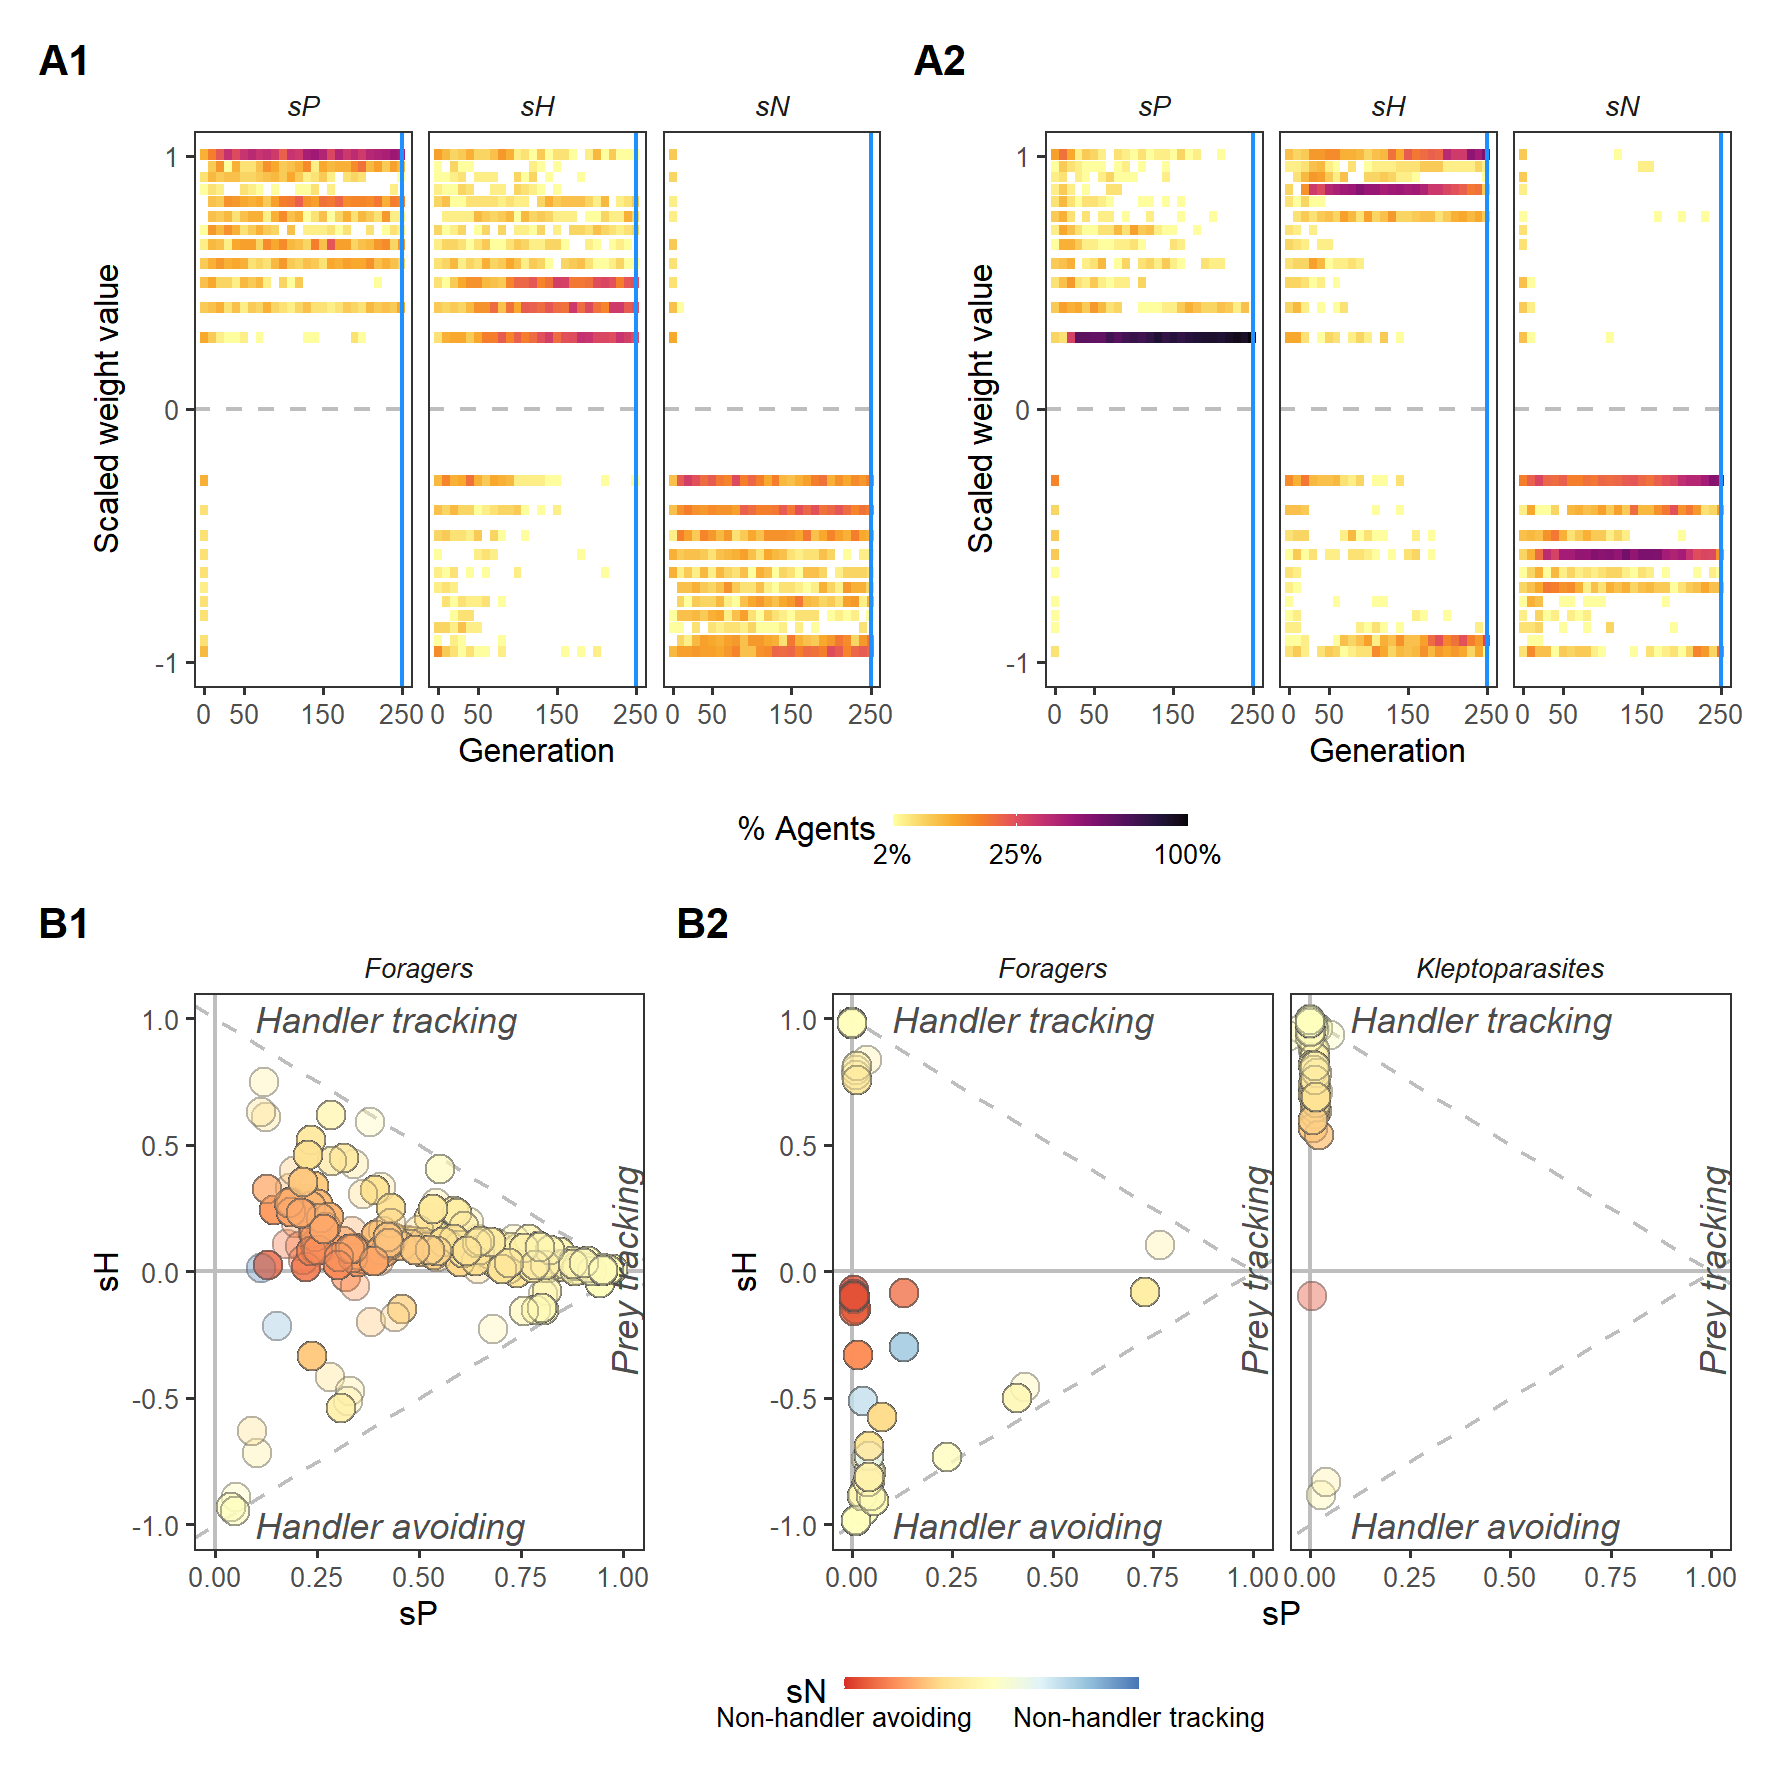
\includegraphics[width=0.90\textwidth]{figures/patternprocess/fig_01.png}
        \caption{
            \textbf{Evolutionary equilibrium and functional variation in movement rules in a spatially explicit, individual-based model of animal movement.}
            We find substantial polymorphism in movement rules in both scenarios of our spatially explicit, individual-based model of the joint evolution of animal movement and competition strategies.
            Agents in both \textbf{(A1)} scenario 1 (exploitation competition only), and in \textbf{(A2)} scenario 2 (fixed, individual competition strategies), evolve multiple, distinct, co-existing values of each of the weights controlling movement rules in the forms of preferences for each cue: $s_P$ (prey-items), $s_H$ (agents handling prey, `handlers'), and $s_N$ (idle agents, `non-handlers').
            The morphs persist across generations, indicating that they likely have equivalent foraging success, and hence, fitness outcomes.
            \textbf{(B1)} In the exploitation competition scenario, the evolved population (at G = 250; blue line in panels A1 and A2) has wide individual variation in their relative preferences for environmental cues (the scaled weights $s_P, s_H, s_N$).
            Most agents trade a preference for prey-items against either an avoidance of non-handlers (orange points), or a preference for handlers (yellow points with $s_H > 0.5$).
            \textbf{(B2)} In the fixed-strategy scenario 2, agents of the two competition strategies (foragers and kleptoparasites) have very different relative preferences for environmental cues.
            While foragers largely either avoid handlers (yellow points, $s_H < -0.5$), or avoid non-handlers (red points), most kleptoparasites prefer moving towards handlers, their direct resource.
            A small number of both foragers and kleptoparasites follow the movement rules of the opposite strategy; these likely represent a strategy mutation during reproduction.
            All panels show simulation runs with $r_{max}$ = 0.01, and show a single replicate for clarity (see the \textit{Supplementary Material} for more replicates).
        }
        \label{fig1}
    \end{figure}
    
    \begin{figure}[h!]
        \centering
        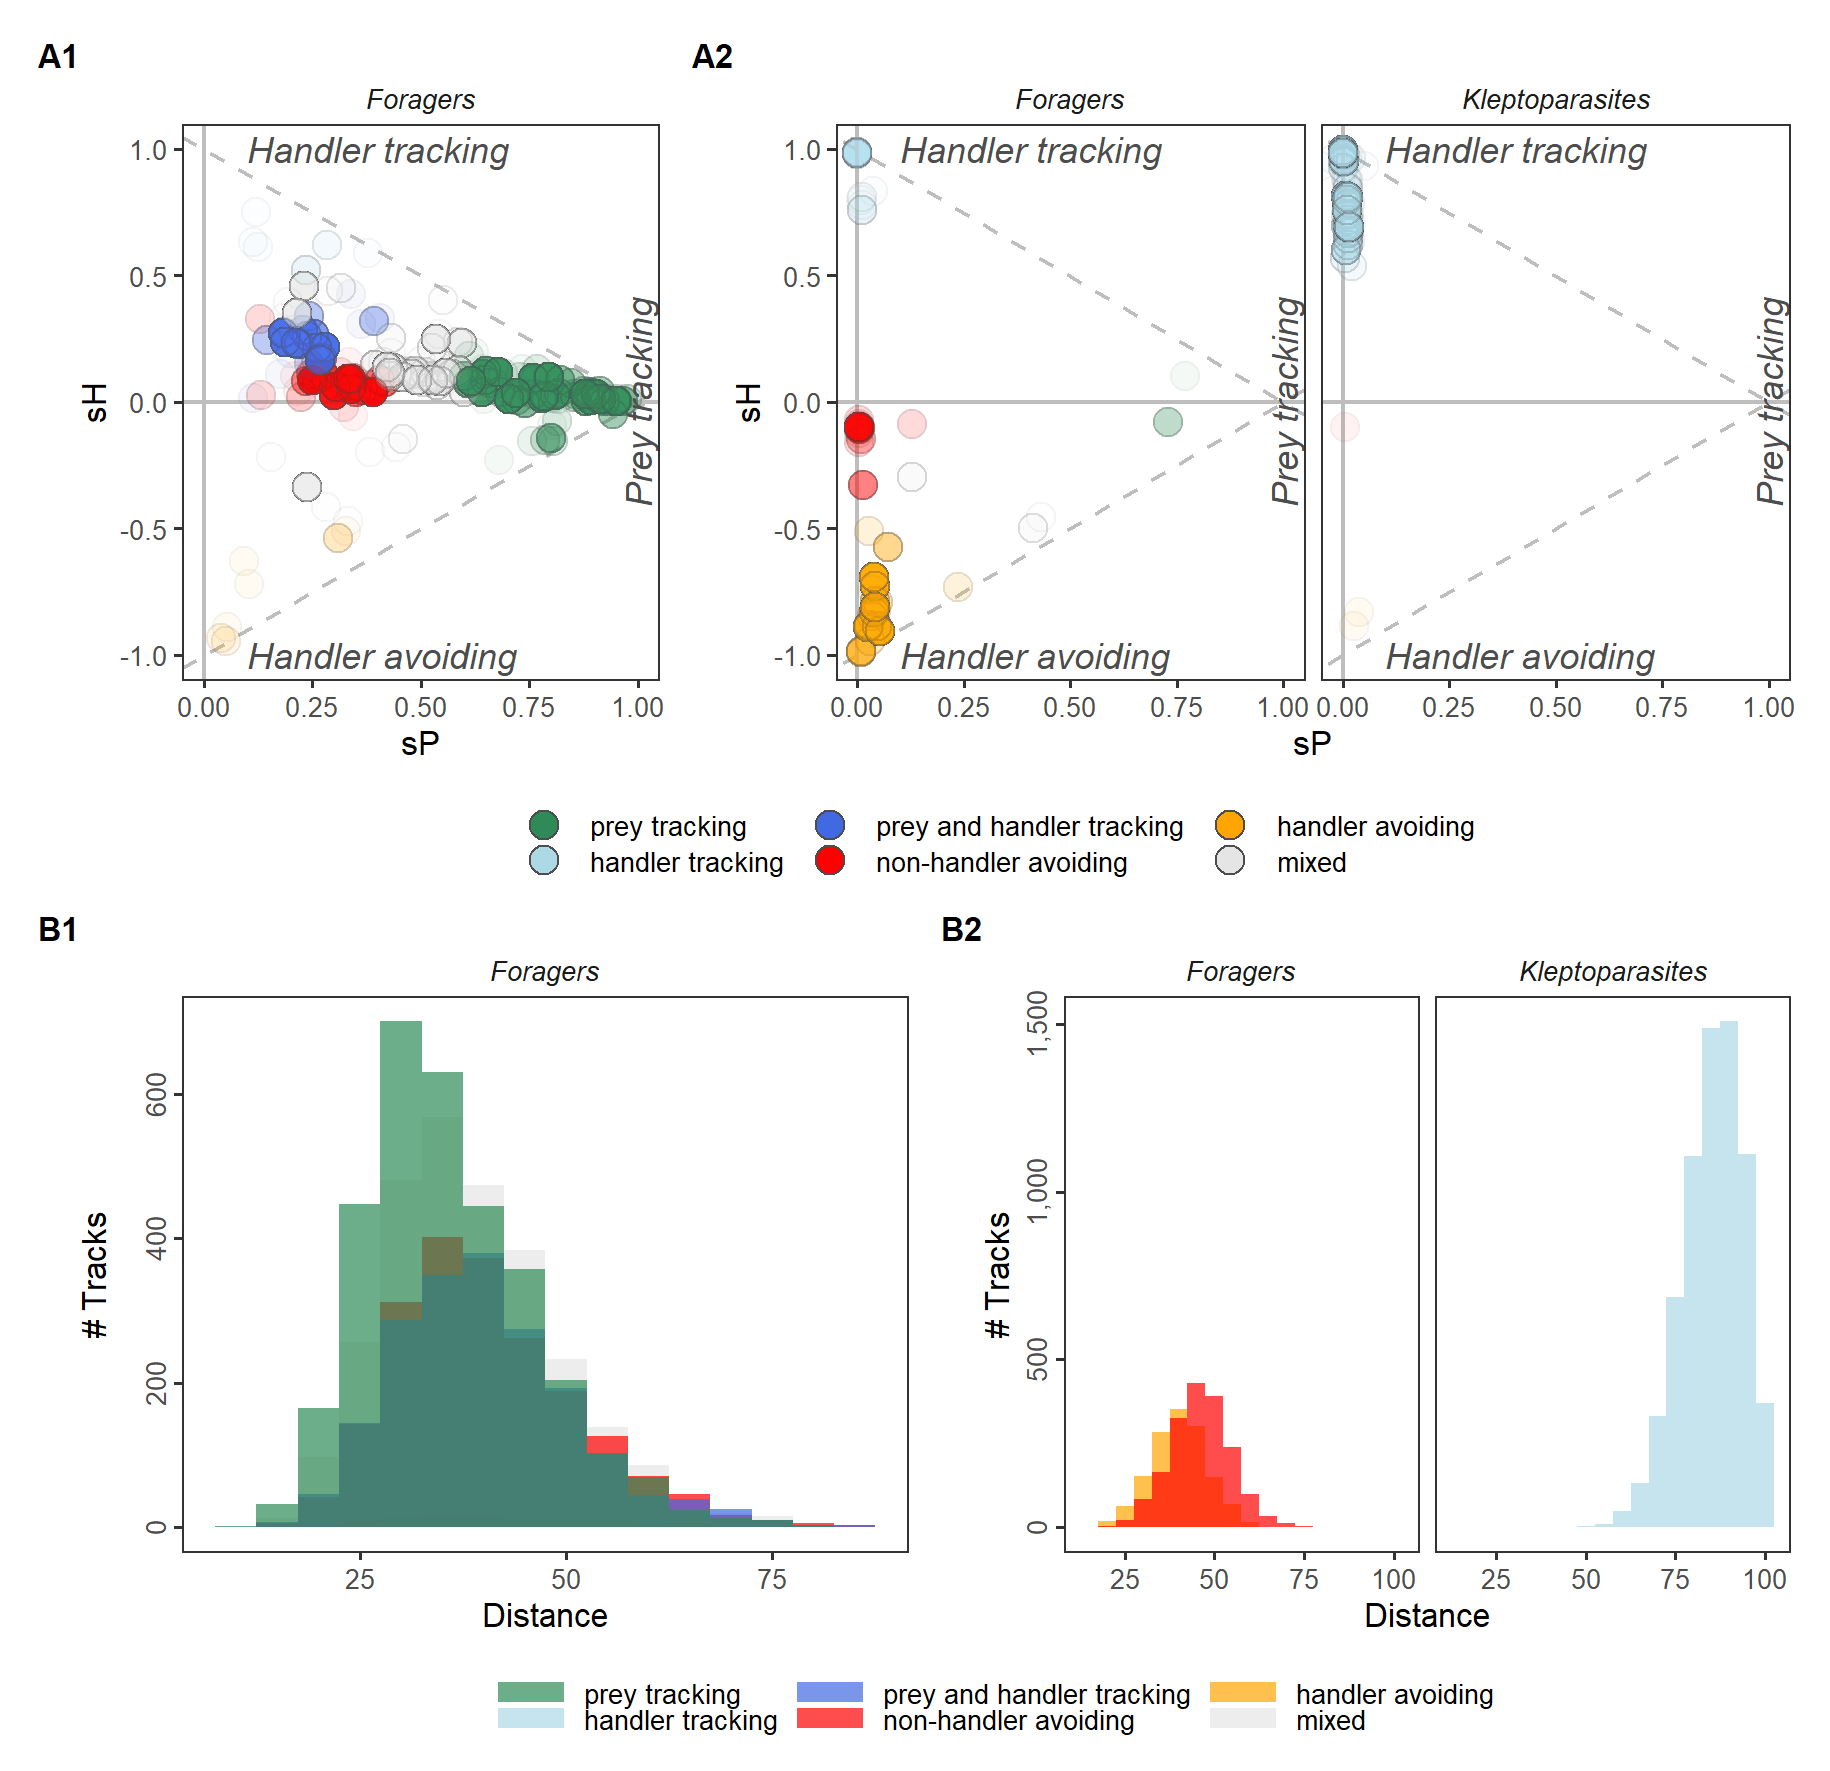
\includegraphics[width=0.90\textwidth]{figures/patternprocess/fig_02.png}
        \caption{
            \textbf{Movement types and competition strategies, and differences in movement paths.}
            We classified agents in both scenario 1 \textbf{(A1)} and scenario 2 \textbf{(A2)} into intuitive `movement types', based on their relative preferences for environmental cues (see Fig. 1 and Main Text). 
            We plotted them based on their weights for prey-items and handlers, adding a transparency to show the frequencies of the types.
            By this simple classification, agents in scenario 1 \textbf{(A1)} mostly track prey-items, or both prey-items and handlers, while avoiding non-handlers.
            Agents in the `mixed' strategy mostly track prey-items and avoid non-handlers.
            In scenario 2 \textbf{(A2)}, most foragers avoid other agents, either handlers or non-handlers; meanwhile, kleptoparasites, as expected, track their primary resource, handlers.
            Regardless of their movement type, agents in \textbf{(B1)} the exploitation scenario all move roughly the same distance in each interval.
            \textbf{(B2)} However, in the kleptoparasitism scenario, the competition strategies differ strongly, with kleptoparasites moving nearly twice as much as foragers.
            Despite moving according to quite different rules (avoid handlers, or avoid non-handlers), both types of foragers move nearly the same distance on average.
            While kleptoparasites' greater movement should be expected to lead to less time for handling prey, and hence lower intake, they save on this time by taking advantage of pre-handled items stolen from foragers.
            Panels A1 and A2 show 5,000 individuals from a single replicate of each scenario, while panels B1 and B2 show the mean movement distance of 100 agents over segments of 100 timesteps from all 10 replicates.
        }
        \label{fig2}
    \end{figure}
    
    \subsection*{Movement Cues, Competition Strategies, and Repeatability of Movement Distance}
    
    Our simulation's populations, at the eco-evolutionary equilibrium (G = 250) were comprised of individuals with a broad range of movement strategies (Fig. \ref{fig3}A).
    In \textbf{scenario 1}, a wider range of movement strategies were evolved on higher productivity landscapes ($r_{max}$ $\in$ 0.02, 0.03), than on lower productivity landscapes ($r_{max}$ = 0.01); the pure handler-tracking and handler avoiding strategies were seen only at at higher growth rates (Fig. \ref{fig3}A1).
    This suggests that on higher productivity landscapes, a wider range of movement types have equivalent fitness.
    The mechanism enabling this is the increased abundance of prey-items: as more agents find prey more easily and become handlers, the relative strength and frequency of the handler cue increases, and navigating using this social information alone becomes a viable movement strategy.
    
    The repeatability of movement distance is nearly five times as high on more productive landscapes ($r_{max}$ $\in$ 0.02, 0.03; repeatability $\approx$ 0.70), as on low productivity landscapes ($r_{max}$ = 0.01; repeatability $\approx$ 0.15; Fig. \ref{fig3}B1).
    This large difference may be because there are more movement types on high-productivity landscapes (Fig. \ref{fig3}A1), with subtle differences in distance moved among them.
    Yet, another plausible explanation is that on high productivity landscapes, there are simply more movement cues, in the form of prey-items and handlers.
    Since the movement types differ in how they process and respond to cues, movement on landscapes with more cues might better reveal subtle differences among the behavioural types.
    
    In \textbf{scenario 2}, increasing productivity also allows a wider range of forager, but not kleptoparasite, movement strategies (Fig. \ref{fig3}A2).
    At the index $r_{max}$ of 0.01, foragers are mostly agent avoiding, while kleptoparasites are handler tracking.
    However, with increasing growth rates, the frequency of kleptoparasites decreases, until, at $r_{max}$ = 0.03, kleptoparasites are extinct in nearly all simulation replicates.
    Thus, on high productivity landscapes, the scenario 2 population is functionally identical to the scenario 1 population, and all individuals follow a forager strategy (see also \citealt{gupte2021a}).
    
    Repeatability analyses on the movement distances of scenario 2 populations is sensitive to how the differences in competition strategy are treated, but not to landscape productivity (Fig. \ref{fig3}B2). Specifically,
    \textit{(1)} When repeatability analysis ignores differences in competition strategy, our populations, comprised largely of handler and non-handler avoiding foragers, and handler tracking kleptoparasites, had repeatability scores $>$ 0.8 (Fig. \ref{fig3}B2a).
    This would suggest that nearly all the variance in movement distance not explained by the fixed effect of environmental productivity is due to between-individual differences (which we know to be primarily differences in competition strategy).\\
    %%
    \textit{(2)} When competition strategy is included as a fixed effect in repeatability analysis, repeatability scores drop substantially to $<$ 0.5 (Fig. \ref{fig3}B2b).
    This suggests that while competition strategies are important in explaining differences in movement distance, a substantial chunk of the unexplained variance is comprised of between-individual variance.\\ 
    %%
    \textit{(3)} Finally, in another plausible way of treating data when the existence of competition strategies is known, running separate repeatability analyses for foragers and kleptoparasites reveals very different repeatability scores for the two strategies (Fig. \ref{fig3}B2c).
    While foragers have repeatabilities betwen 0.0 and 0.75, depending on the growth rate, kleptoparasites have repeatabilities close to zero.
    
    There did not appear to be an effect of landscape productivity as in scenario 1.
    This may be because, in scenario 2, the presence of kleptoparasites (indeed, as the majority strategy) reduces prey-item extraction from the resource landscape.
    Consequently, all scenario 2 landscapes eventually resemble scenario 1 landscapes at $r_{max}$ = 0.03.
    We ran analyses only on growth rates of 0.01 and 0.02, as kleptoparasites rapidly go extinct early on in simulations with a growth rate of 0.03 \citep[see][for an explanation of the evolutionary dynamics]{gupte2021a}.
    
    \begin{figure}[h!]
        \centering
        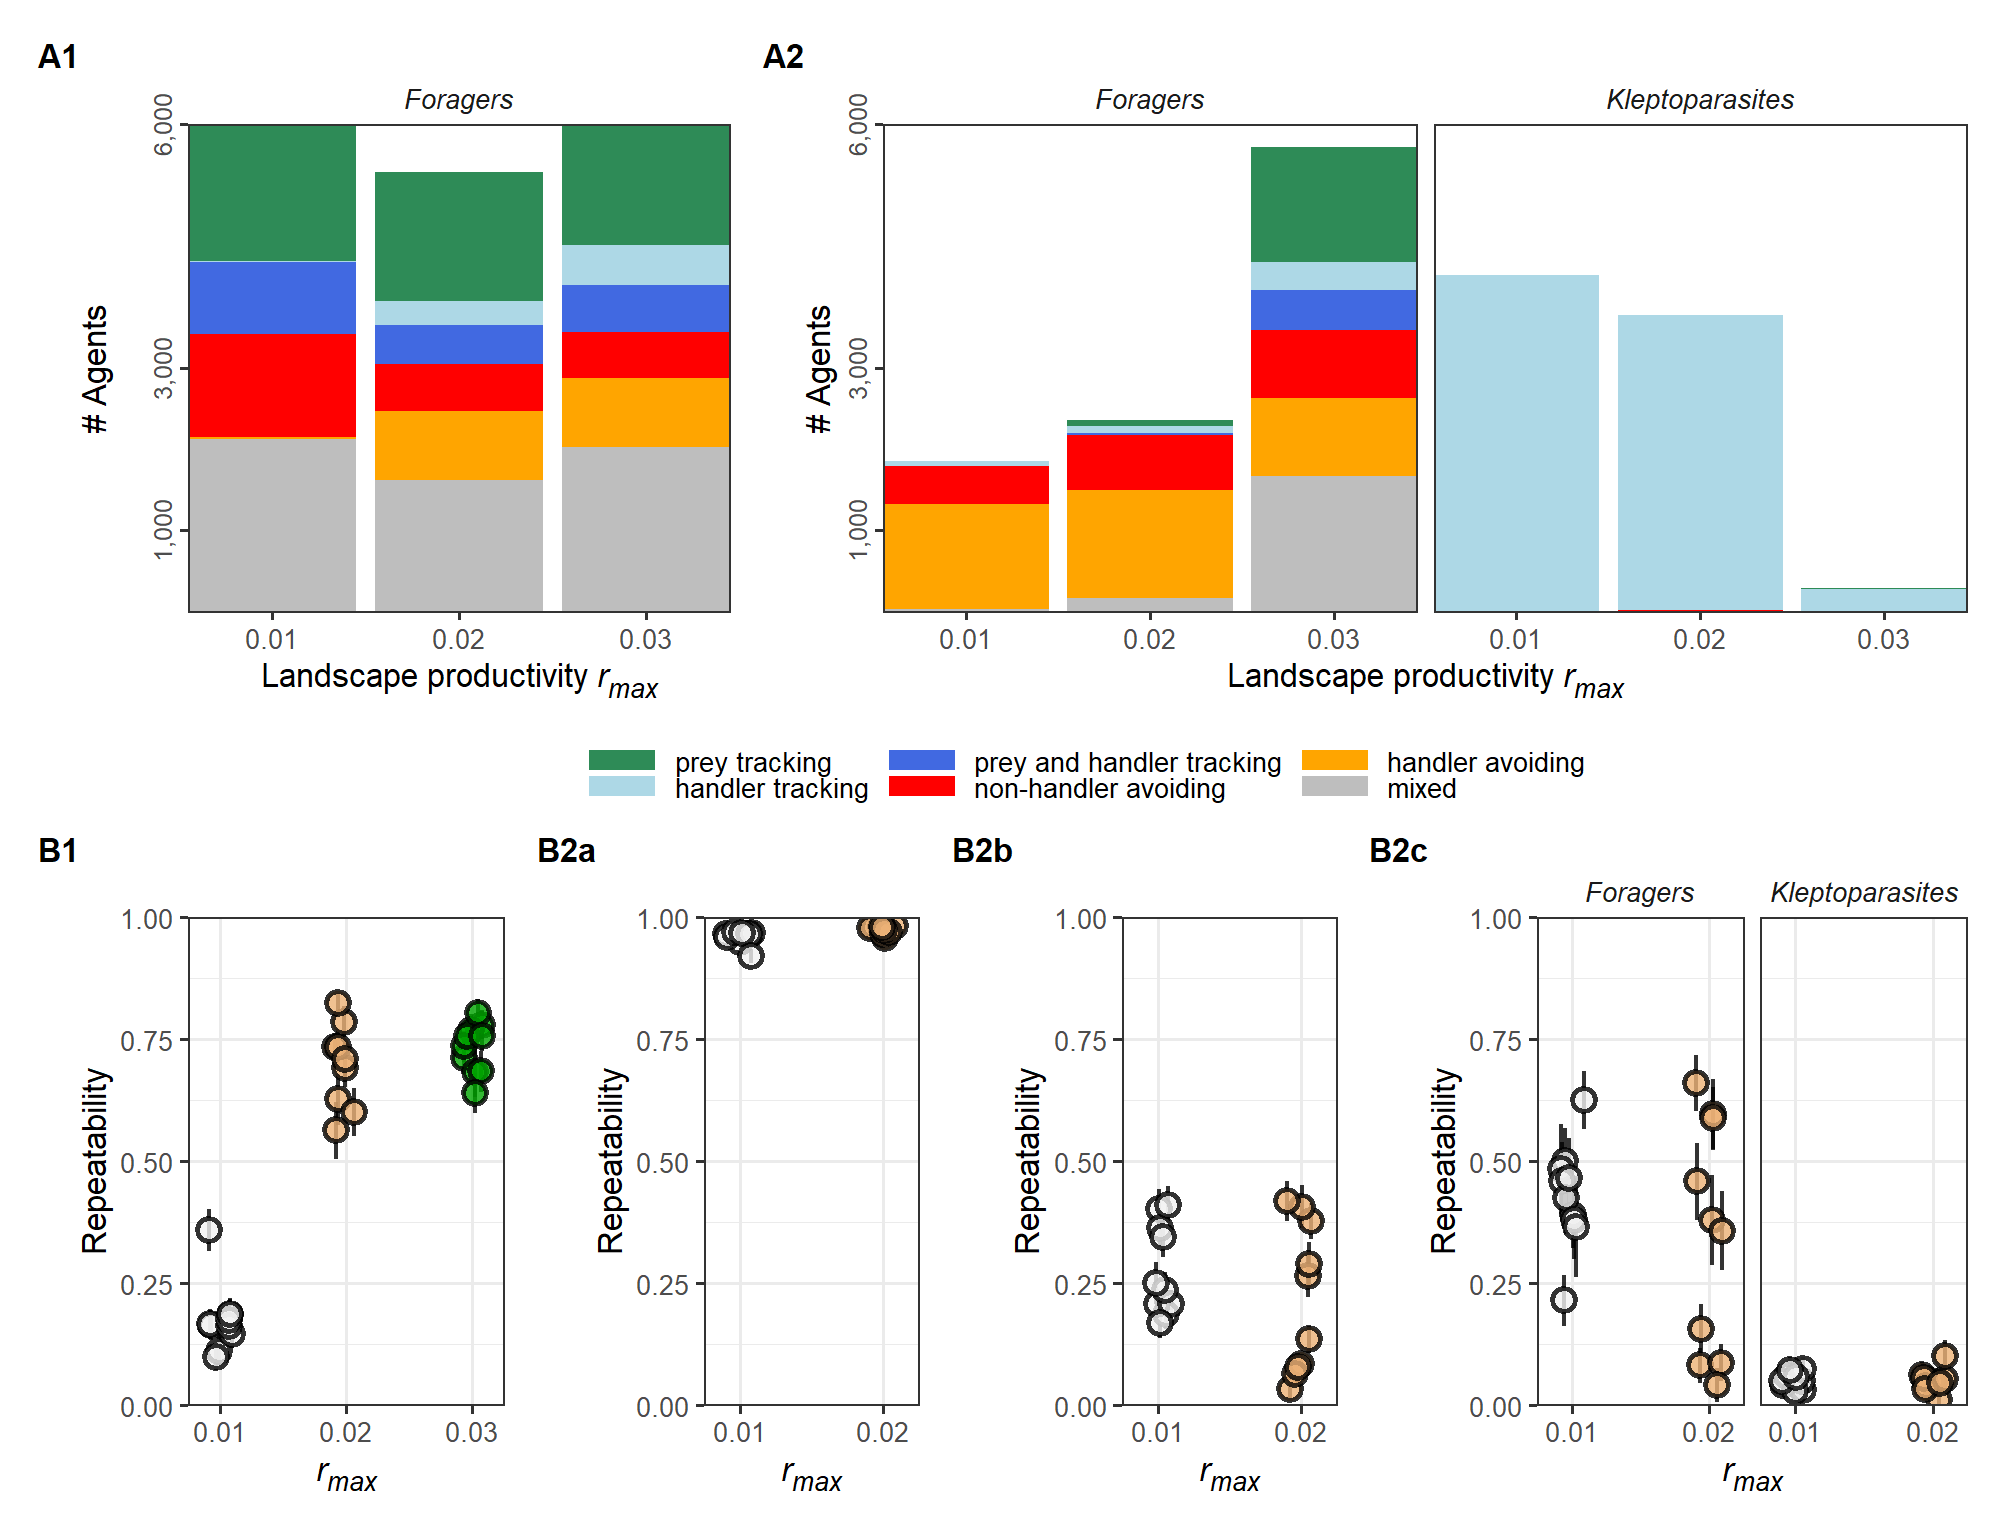
\includegraphics[width=1.0\textwidth]{figures/patternprocess/fig_03.png}
        \caption{
            \textbf{Frequency of movement types, competition strategies, and environmental cues, and consequences for repeatability analyses to detect individual differences in movement.}
            Increasing landscape productivity ($r_{max}$) beyond the index value of 0.01 leads to more prey-items on the landscape, and hence more available cues for movement decisions.
            In \textbf{(A1)} scenario 1, this leads to a change in the frequencies of movement types, with the persistence of handler-avoiding and pure handler-tracking types.
            In \textbf{(A2)} scenario 2, the frequencies of both movement types and competition types change with the increased availability of prey-items: at higher $r_{max}$ (0.03), foragers are both more common, and use more movement strategies, than at lower $r_{max}$ (0.01).
            The repeatability of movement distance is greater for scenario 1 populations on landscapes with higher $r_{max}$, and hence more available movement cues \textbf{(B1)}.
            This suggests that individual differences in movement decision-making mechanisms may be more readily detected when agents are actually able to process environmental cues using those mechanisms, rather than when agents move on relatively `clueless landscapes'.
            When agents' competitive strategy strongly influences their movement, as in scenario 2 \textbf{(B2 panels)}, repeatability analyses are strongly affected by how this difference is treated.
            \textbf{(B2a)} If differences in competitive strategies are not included in the model formulation, repeatability scores are consistently high ($>$ 0.9).
            \textbf{(B2b)} When agents' competitive strategy is included as a fixed effect, repeatability scores are substantially lower ($< 0.5$).
            Finally, \textbf{(B2c)}, repeatability models run separately for each of the competitive strategies would essentially reveal that competitive types with strong dimorphism (or clustering) in movement types (here, foragers) have a higher repeatability than competitive types with a monomorphic movement strategy (here, kleptoparasites).
            Panels A1 and A2 show frequencies pooled over 100 agents from 10 replicate simulations, with agent data exported at G = 200, 210, \ldots 249.
            Panels B1 and B2 used long-term movement paths from 100 agents in generation 250, over 10 replicates. B2 omits $r_{max}$ = 0.03, as kleptoparasites are often extinct.
        }
        \label{fig3}
    \end{figure}
    
    \subsection*{Individual Differences in Habitat Selection}
    
    We fit 6,000 step-selection functions to thinned movement data from 60 simulation runs, with 10 replicates for each $r_{max}$ value (0.01, 0.02, 0.03) and scenario (1 and 2).
    In \textbf{scenario 1}, all agents forage and have a substantial preference for moving towards prey-items.
    Consequently, the estimated coefficients of their apparent selection for cell productivity $r$ are all positive, with no differences among the movement strategies (Fig. \ref{fig4}A1, B1).
    On the other hand, in \textbf{scenario 2}, the dramatic difference in competition strategies is reflected in the estimated coefficients of apparent selection for cell $r$; foragers have substantially lower (and even negative) selection for $r$ than kleptoparasites (Fig. \ref{fig4}A2).
    However, there is little difference between foragers moving mostly to avoid handlers or to avoid non-handlers (Fig. \ref{fig4}B2).
    %%
    As landscape productivity increases, scenario 2 populations, but not scenario 1 agents, show a shift in their selection for cell $r$.
    At higher growth rates ($r$ = 0.02), scenario 2 populations --- still comprised of about equal proportions of foragers and kelptoparasites (see Fig. \ref{fig3}) --- show substantially more overlap between the two strategies' selection for $r$ (Fig. \ref{fig4}A2).
    This is carried over as an overlap between the three main movement types (Fig. \ref{fig4}B2).
    At the highest growth rates, scenario 1 and scenario 2 populations are essentially identical, and the few kleptoparasites remaining in scenario 2 apparently select for $r$ similar to foragers.
    Overall, applying step-selection analysis to our model output suggests that differences between competition strategies, when associated with different movement types, could be revealed under certain conditions from animal movement paths.
    
    \begin{figure}[h!]
        \centering
        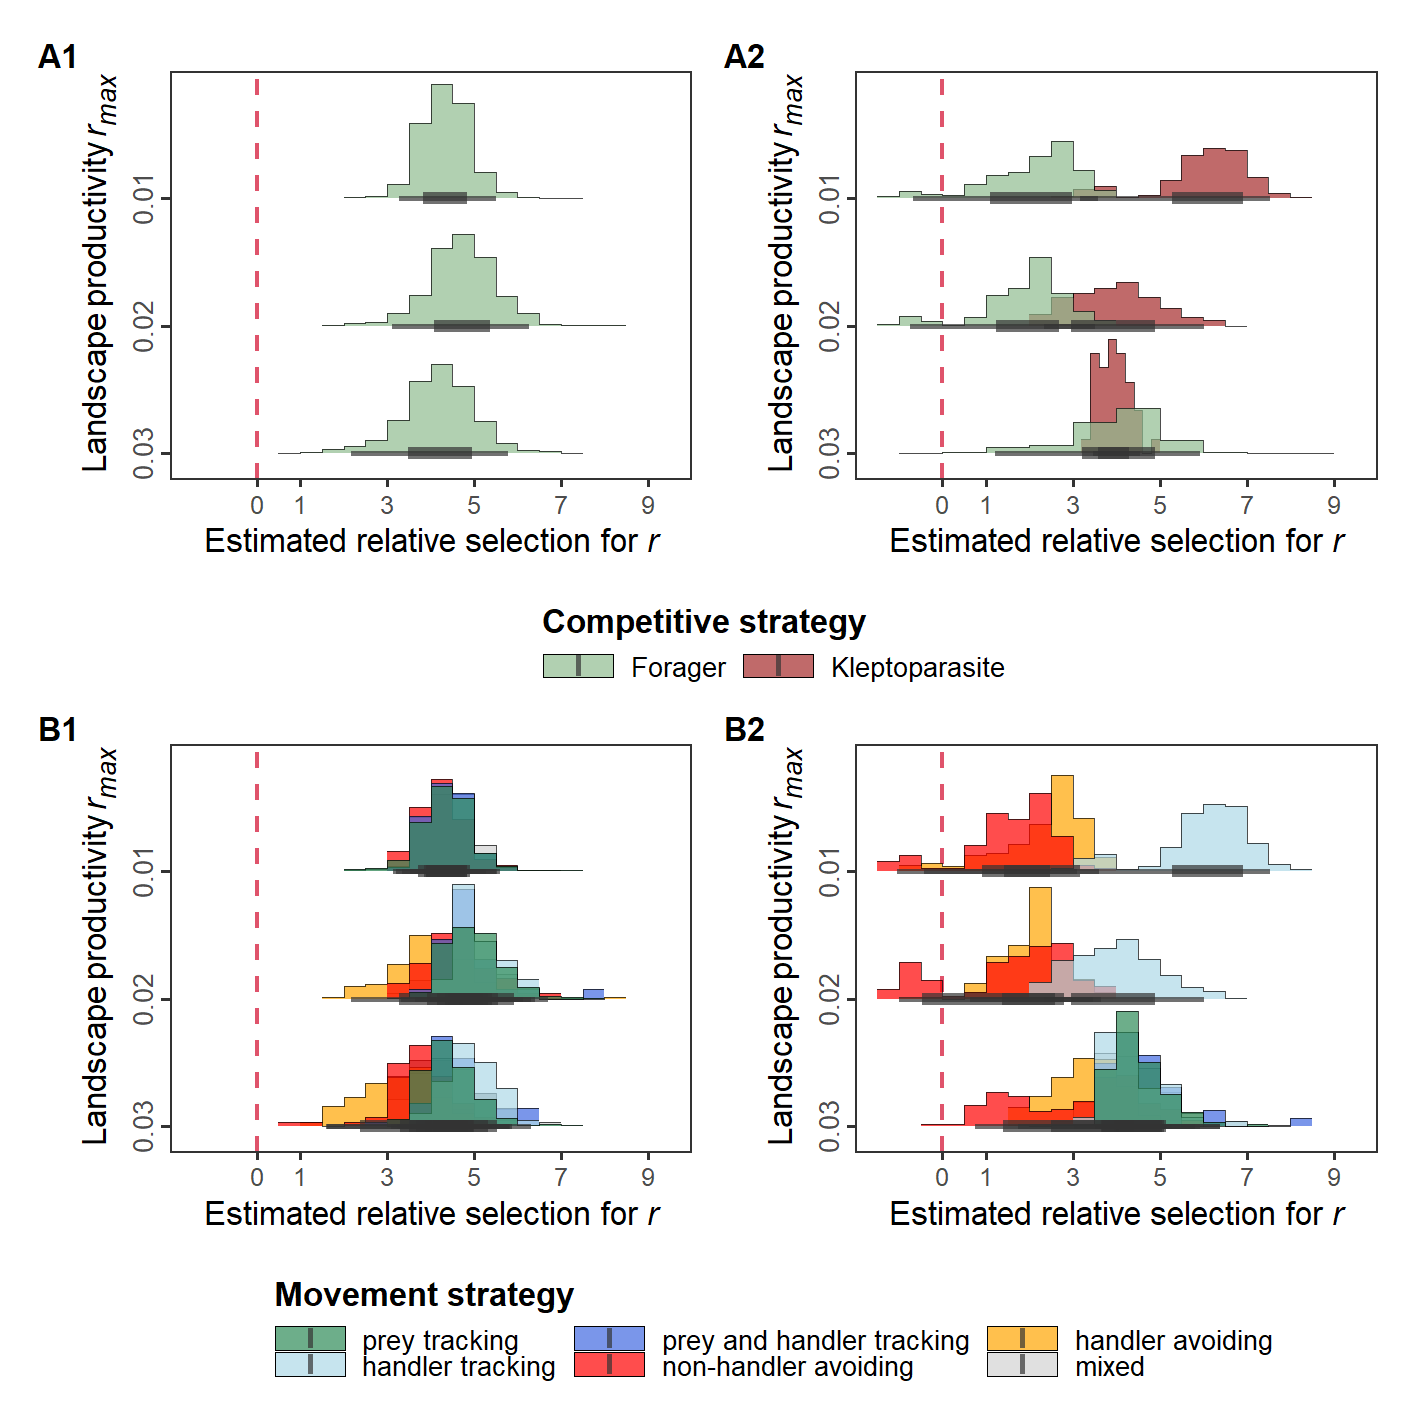
\includegraphics[width=0.90\textwidth]{figures/patternprocess/fig_04.png}
        \caption{
            \textbf{Movement types and competition strategies revealed in step-selection analyses.}
            Applying step-selection analysis to long-term movement paths from \textbf{(A1)} scenario 1, and \textbf{(A2)} scenario 2 reveals strong differences in apparent selection for landscape productivity between competition strategies ($r_{max}$ = 0.01).
            In \textbf{(B1)} scenario 1 and \textbf{(B2)} scenario 2, the apparent selection strengths for productivity $r$ of foragers of different movement types overlaps.
            Handler-tracking kleptoparasites in scenario 2, too, have apparent selection strengths for $r$ that overlap with those of some foragers, but which are substantially higher than those of most foragers, which avoid both handlers and non-handlers. 
            These essentially opposing movement strategies are picked up as differences in selection for $r$.
            Kleptoparasites track handlers, and the probability of a forager finding prey and handling are higher at the centres of resource peaks, i.e, cells with high $r$.
            Conversely, foragers avoid other agents, and since high-productivity cells are more likely to have agents, they apparently select \textit{against} high productivity cells.
            All panels show selection coefficients from 100 agents' long-term movement paths at G = 250, from 10 replicates of each simulation; only coefficients with $p \leq$ 0.05 are shown.
        }
        \label{fig4}
    \end{figure}
    
    \section{Discussion}
    
    % % Detecting Individual Consistency from Agent Paths
    
    We used an evolutionary individual-based model of animal movement decision-making under two scenarios of foraging competition (\textit{Kleptomove}; \citealt{gupte2021a,netz2022a}), to investigate what we can learn about individual-differences by applying statistical analyses to animal movement data.
    % %%
    % We showed that the model, as expected, reached an ecological equilibrium in mean per-capita intake, as well as the mean per-capita distance moved.
    Our evolved agent populations showed substantial between-individual differences in their relative preferences for environmental cues (`movement types'; \citealt{getz2015}): when presented with the same cues, agents could make substantially different decisions about where to move.
    %%
    We showed that despite very different relative differences among the movement types for environmental cues, the types did not consistently differ in their movement distance.
    However, in our scenario 2, in which individuals had a fixed competition strategy (forager or kleptoparasite), kleptoparasites moved much more than foragers.
    %%
    With few between-type differences in movement distance, the repeatability of movement distance was low in scenario 1 at low growth rates, but increased substantially at higher growth rates.
    In scenario 2, not accounting for differences in competition strategy led to repeatability scores $\approx$ 1.0, but correcting for these differences led to lower repeatability scores.
    %%
    Finally, applying step-selection analysis to estimate agents' apparent selection for landscape productivity showed no differences among movement types in scenario 1, but revealed clear differences between competition strategies (and their correlated movement types) in scenario 2.
    %%
    % Our application of relatively simple analyses to a model with highly dynamic agent distributions,arising from simple movement rules and foraging mechanisms, emphasise the challenge in relating animals' behavioural mechanisms to the movement paths that are their outcomes.
    
    \subsection*{Variation Among Movement Types and Competition Strategies}
    
    The co-existence of multiple movement types across multiple generations of scenario 1 suggests that multiple alternative movement rules are equally good for navigating our fluctuating resource and social landscapes \citep[see also][]{getz2015,netz2020}.
    That movement types travel roughly the same distances is not surprising, as they must spend the same time handling, and gaining intake, to have equivalent fitness.
    In scenario 2, there are essentially only two viable movement types that are strongly correlated with competition strategies at low growth rates ($r_{max}$ = 0.01).
    Here, the handler-tracking kleptoparasites move more because their primary resource, handlers, are scarce; conversely, foragers move less, as prey-items are abundant \citep[see][]{gupte2021a}.
    Yet both strategies have equivalent fitness because kleptoparasites make up for lost time by having to handle stolen prey-items for a shorter duration.
    We suggest that for movement types to differ in their path metrics (e.g. distance, or speed; see \citealt{abrahms2017}), between-individual variation and within-individual consistency along a further axis of behaviour that equalises fitness between the types is likely necessary.
    
    \subsection*{Repeatability Analysis}
    
    Repeatability analysis of the scenario 1 movement paths showed that populations evolved on higher productivity landscapes had significantly higher repeatability scores.
    The major difference between lower ($r_{max}$ = 0.01) and higher productivity landscapes ($r_{max}$ = 0.03) is that the latter have many more prey-items per cell.
    While agents on low growth rate landscapes often encounter areas with few or no movement cues (`clueless regions'; \citealt{perkins1992}), this is much more rarely the case on high productivity landscapes.
    Since our agents' decision-making mechanisms --- in common with animal cognitive systems --- require environmental cues to make movement decisions, between-individual differences in movement are more readily detected on landscapes with more movement cues \citep[see][]{carter2013a}.
    Our result might suggest that populations with different movement types transplanted between information-poor and information-rich landscapes would show a marked increase in behavioural consistency.
    We caution against this interpretation, as our populations have \textit{evolved}, rather than simply been tested on, landscapes across a productivity gradient.
    On high productivity landscapes, a wider range of movement types is evolved, highlighting how measures such as repeatability are linked to the evolutionary trajectory of populations.
    
    Using scenario 2, we illustrated three different ways of implementing repeatability analysis for a population with correlated differences in movement type and competition strategy.
    When differences in competition strategy were ignored, repeatability scores were close to 1.0, as the variance in movement distance due to competition strategy was picked up as between-individual variance instead.
    Adding competition strategy as a fixed effect to the analysis resulted in lower repeatability values; this was expected, as differences among competition strategies explain the bulk of the variance.
    Finally, performing separate repeatability analyses for foragers and kleptoparasites yielded very low repeatability scores for kleptoparasites, which foragers were still quite repeatable.
    This last result is potentially because kleptoparasites are solidly monomorphic in their movement type, while foragers may be either handler- or non-handler-avoiding, and this difference in decision-making mechanism could result in subtle differences in movement metrics.
    Overall, we suggest that extremely high repeatability scores might indicate that an important source of variation is not being taken into account, and should be sought for.
    Multivariate methods can help identify within-individual behavioural co-variation in movement metrics, such as distance and displacement \citep{hertel2019,hertel2021}.
    This approach could help reveal strong associations between movement types and competition strategies, as in our model, or responsiveness to social cues \citep{strandburg-peshkin2015}.
    Identifying such behaviours from animal movement data is likely to require very high-resolution tracking and associated computational methods (Nathan et al. \textit{in prep.}).
    
    \subsection*{Individual Differences in Habitat Selection}
    
    In a novel application of step-selection analysis to the study of individual differences, we showed that agents of different competition strategies (scenario 2), but not of different movement types (both scenarios 1 and 2), had diverging selection for environmental conditions.
    An important reminder is that our model's agents cannot actually detect cell productivity $r$, and therefore the preference for $r$ values is more correctly termed apparent selection.
    This situation parallels empirical analysis of animal tracking data, in which researchers commonly use long-term indices of environmental conditions (e.g. NDVI; \citealt{pettorelli2011}) to approximate the ephemeral movement cues actually encountered and acted upon by individuals.
    Nonetheless, strong between-individual differences (here, in competition strategy) are likely to be reflected in animals' apparent selection for environmental conditions.
    In our model, the difference in apparent selection arises from the distribution of movement cues relative to cell growth $r$.
    Handler-tracking kleptoparasites have a higher selection for $r$ because high-$r$ cells are more likely to have handlers, since foragers are more likely to find prey-items there and begin handling.
    On the other hand, agent-avoiding foragers have a lower selection for $r$ as they avoid resource peaks, which are more likely to have more agents.
    Some foragers will always be found on high-$r$ cells, as even a forager moving across the landscape at random (which they do not) is more likely to stop and begin handling on a high-$r$ cell than a cell at the periphery of a resource peak.
    
    \subsection*{Individual-based Models as a Check on Statistical Methods}
    
    Individual-based models are not new in movement ecology, and are increasingly used and prescribed to better understand animal movement \citep[see a review in][]{deangelis2019}.
    Such models have been used to illustrate the importance of animal movement to phenomena such as disease outbreaks \citep{white2018}, and sympatric speciation \citep{getz2015}, while also showing how individual differences in animal movement strategies can have downstream effects on population-level phenomena such as habitat-selection and social interactions \citep{spiegel2017,spiegel2016a}.
    There is also a rich tradition of individual-based models being used to assess the performance of methods intended for use on empirical tracking data.
    For example, \citealt{gurarie2016}, \citealt{michelot2016}, and \citealt{patin2020a} simulated the paths of individuals with different behavioural modes to test the performance of tools to detect behavioural change-points, where the animal switches from one movement mode to another.
    However, very few individual-based models that are used as checks on statistical methods actually model the fine-scale decisions --- comprising comparisons among, and eventual selection of --- steps that comprise animal movement \citep[but see recently][]{vissat2021}.
    This is at least partially because few statistical methods seek to estimate animal movement preferences, and by implication, animal cognitive processes, at such fine scales.
    Step-selection analysis has the potential to be among these methods, as it directly links what animals actually perceive, to where they go \citep[see recently][]{aben2021}.
    This allows a fine-scale comparison between selected and alternative steps, which, at certain scales, may functionally approximate individuals' cognitive processes, at least in terms of preference or avoidance.
    
    Our model \citep{gupte2021a,netz2022a} and other mechanistic individual-based models that follow similar principles \citep{getz2015,getz2016,netz2020}, allow for the implementation of different movement decision-making mechanisms at very fine scales, in biologically plausible ways.
    Our agents' movement decisions integrate locally available cues to make adaptive movement decisions, just as real animals are expected to do \citep{nathan2008a}.
    While our agent responses are linear, they can in principle be much more complex, including convoluted relationships between the environmental cues, as well as separate weights for each cue combination.
    Coupled with the ability to know the state of the environment, and of each agent, at any point in the simulation, we believe this and other similar models are suitable for the testing of a range of empirical methods.
    For example, a better test of whether step-selection analysis can determine agent preferences for environmental cues, and individual differences therein, could involve the dynamic logging of selected and alternative steps, as well as the environmental covariates (prey-items and competitors) at those steps, in order to compare between them at fine scales.
    Such logging would immediately reveal that often, agents have either very few direct local cues, or very few differences between conditions at alternative and selected steps, on which to base movement decisions at fine timescales \cite[relatively clueless regions, per][]{perkins1992}.
    This highlights a potential challenge to such analyses from the ever increasing resolution of animal tracking and environmental monitoring data; for example, how should step-selection analysis be adapted to account for high spatial- and temporal-autocorrelation in animals' environments, while still taking advantage of high sampling frequencies.
    
    \section*{Conclusion}
    
    The analysis of our model's agent movement paths using contemporary statistical tools from movement ecology showed that it is often challenging to infer animals' decision-making processes, or even relative differences among individuals, from tracking data alone.
    First, when seeking to assess individual consistency and between-individual differences from animal tracking data, it is key to include predictors that have a mechanistic relationship with the behavioural response being studied.
    For species that are only poorly known, or difficult to study in captivity, this requires first collecting substantial knowledge on natural history and behavioural biology.
    Researchers could potentially apply a model selection approach \citep{burnham2011}, to determine which fixed effects are best suited to their study species.
    Second, uncovering individual behavioural tendencies in captivity may not be sufficient to describe animal movement in natural environments, which is likely to be affected by fine-scale fluctuations in resources, as well as the social environment.
    Finally, attempting to recover animals' movement preferences at fine scales is a challenging task.
    In part, this is due to a mismatch of scales: empirical researchers are rarely able to study fine-scale movement decisions, because suitably fine-scale data on the environmental cues that go into these decisions are not available.
    While increasingly high-resolution animal tracking is becoming more common, there would need to be a concurrent increase in the resolution of environmental monitoring \textit{from the animal's point of view}.
    The availability of such data sources would make the development of statistical tools that account for particular issues --- such as spatio-temporal autocorrelation --- a priority in movement ecology.
    Individual-based models, in which simple mechanisms can give rise to substantial complexity in animal movement and population distributions, could be very useful as test-beds to investigate whether current and upcoming tools are truly capable of parsing patterns to recover the underlying processes.
    
    \section*{Data and Code Availability}
    
    The simulation code for the \textit{Kleptomove} model is on Zenodo as \citealt[(zenodo.org/record/4905476)]{netz2022a}, and on Github: github.com/pratikunterwegs/Kleptomove.
    %
    Simulation data are available from DataverseNL as a draft: \textbf{UPDATE WITH DRAFT DATA}.
    Data will be at this persistent link after publication: \textbf{UPDATE WITH PERSISTENT DOI}.
    Data analysis code is on Github: github.com/pratikunterwegs/pattern-process.
    
    \section*{Acknowledgments}
    
    The authors thank Christoph Netz and Hanno Hildenbrandt for contributing extensively to the coding of the simulation model \textit{Kleptomove};
    Jakob Gismann and other members of the Modelling Adaptive Response Mechanisms Group at the University of Groningen for helpful discussions on the manuscript.
    F.J.W. acknowledges funding from the European Research Council (ERC Advanced Grant No. 789240).
    P.R.G was supported by an Adaptive Life Programme grant made possible by the Groningen Institute for Evolutionary Life Sciences (GELIFES).

    \newrefcontext[sorting=nyt]
    \section*{Literature Cited}
    \printbibliography[title=Literature~Cited,heading=none]
\end{refsection}
